\section{Evaluation}
\label{results}

We next measure Thermostat's automatic hot/cold classification and run-time
placement/migration mechanisms on our suite of cloud applications.

Thermostat takes as input a tolerable slowdown; a single input parameter 
specified by a system administrator.  It then automatically selects cold pages
 to be migrated to slow memory at runtime. We set a tolerable slowdown of
3\% throughout our evaluation, since a higher slowdown may lead to an overall
cost increase due to higher required CPU provisioning (which is more expensive
than memory). Thermostat's slowdown threshold can be 
changed at runtime through the Linux cgroup mechanism. Hence,
application administrators can
dynamically tune the threshold based on service level agreements
for latency-critical applications or for the throughput requirements of
batch jobs.  We show that, for our application suite, Thermostat meets the
target 3\% slowdown while placing a significant fraction of application footprint in slow memory
dynamically at runtime.

%Based on the characterization results shown in Figure~\ref{fig:cassandra-hotspot},
%we set an objective of migrating roughly half of the application memory footprint
%to slow memory with an expected performance degradation of 5\% for Cassandra
%and TPCC.  However, for Redis, the memory access locality pattern is flat, and
%a 5\% degradation target allows only a small fraction of the footprint to be classified
%as cold.  Hence, for Redis, we set a 10\% degradation target.

We evaluate Thermostat with 5\% of huge pages sampled in every scan interval of
30s and at most 50 4KB pages poisoned for a sampled huge page.
We compare the performance of Thermostat with a placement policy that
places all pages in DRAM, which maximizes performance while incurring maximal 
memory cost.  Thermostat's sampling mechanisms incur a negligible performance
impact (well under 1\%)---the slowdowns we report are entirely attributable to 
slow memory accesses. 

We briefly discuss our findings for each application. Table~\ref{tab:memory-footprint} reports each 
application's footprint in terms of resident set size (RSS) and file-mapped
pages. The memory savings quoted for each benchmark is the average cold memory
fraction over the benchmark's runtime.

\begin{figure}[t]
\centering
%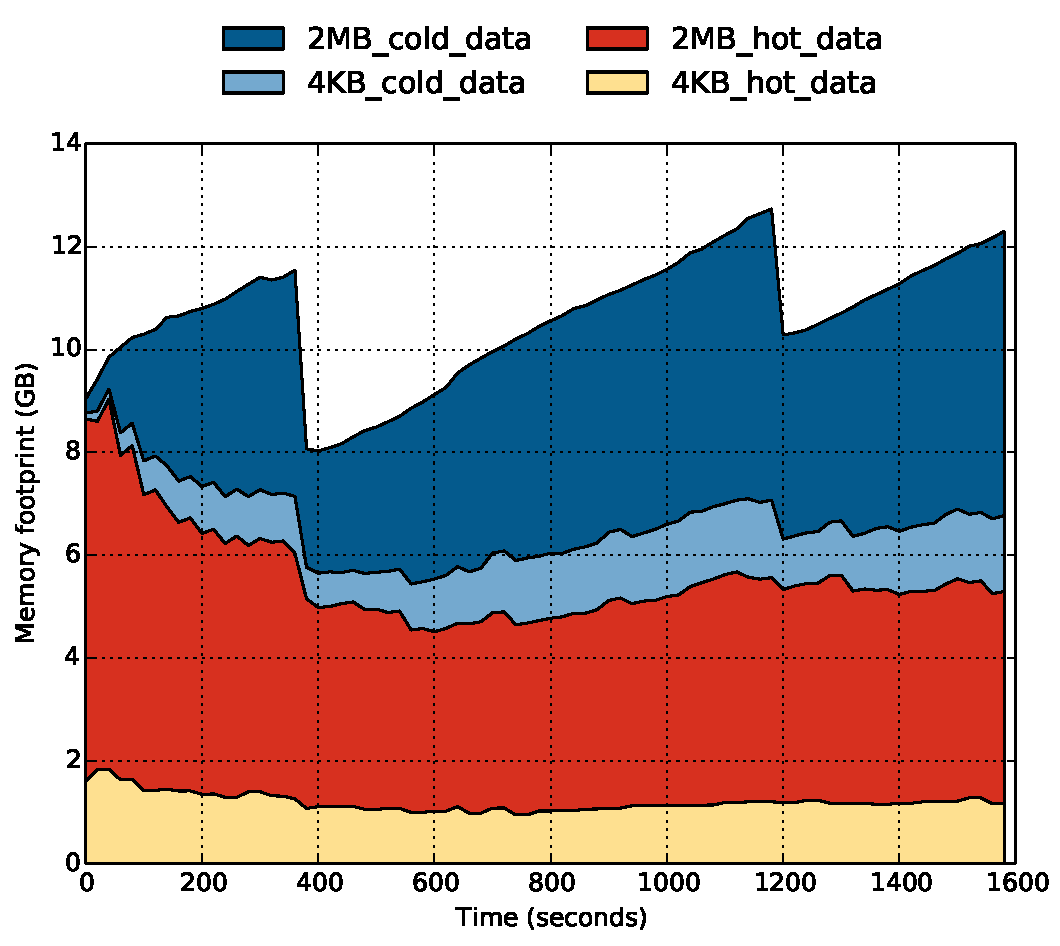
\includegraphics[width=1.0\columnwidth]{figures/cassandra-capacity.pdf}
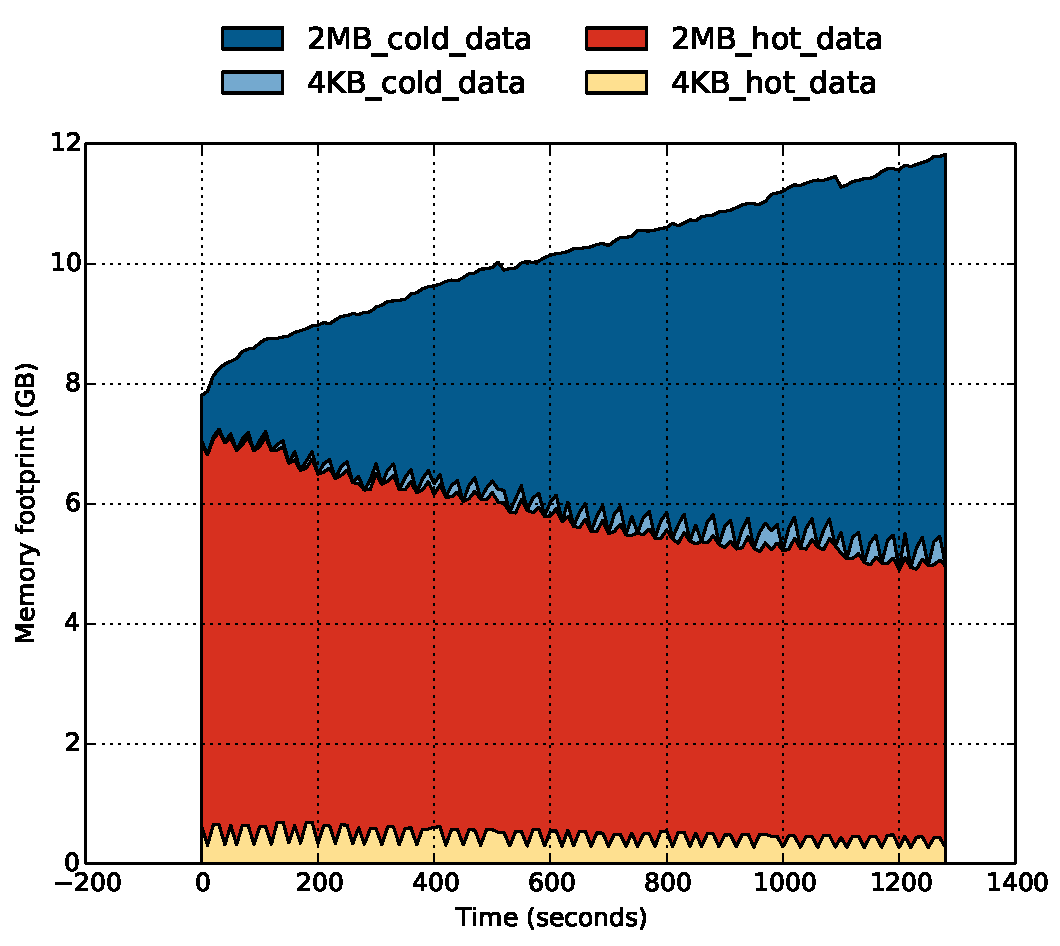
\includegraphics[width=0.8\columnwidth]{asplos2017/figures/cassandra-new-set-policy-kstaled10-sample5-period3-capacity_over_time.pdf}
\caption{Amount of cold data in Cassandra identified at run time with 2\%
throughput degradation for a write-heavy workload (5:95 read/write ratio).}
\label{fig:cassandra-capacity}
\end{figure}

\begin{figure}[t]
\centering
%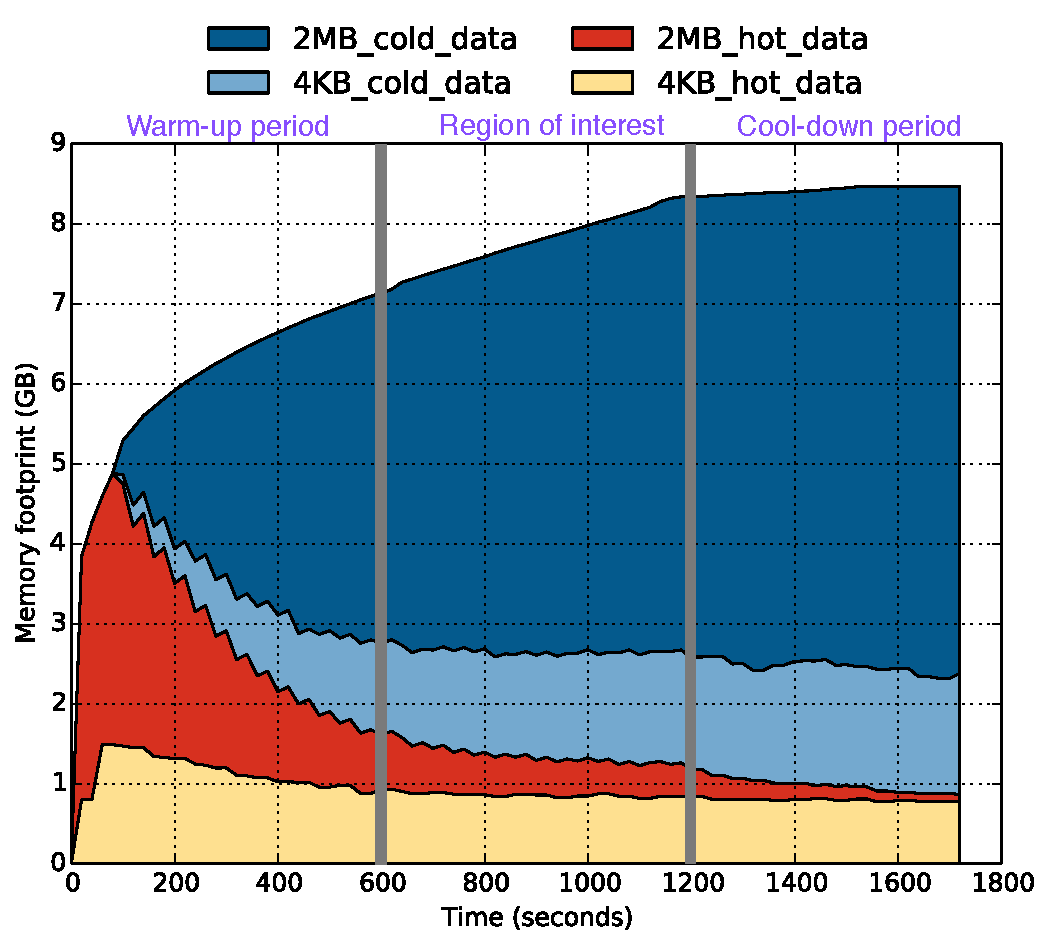
\includegraphics[width=1.0\columnwidth]{figures/tpcc-capacity.pdf}
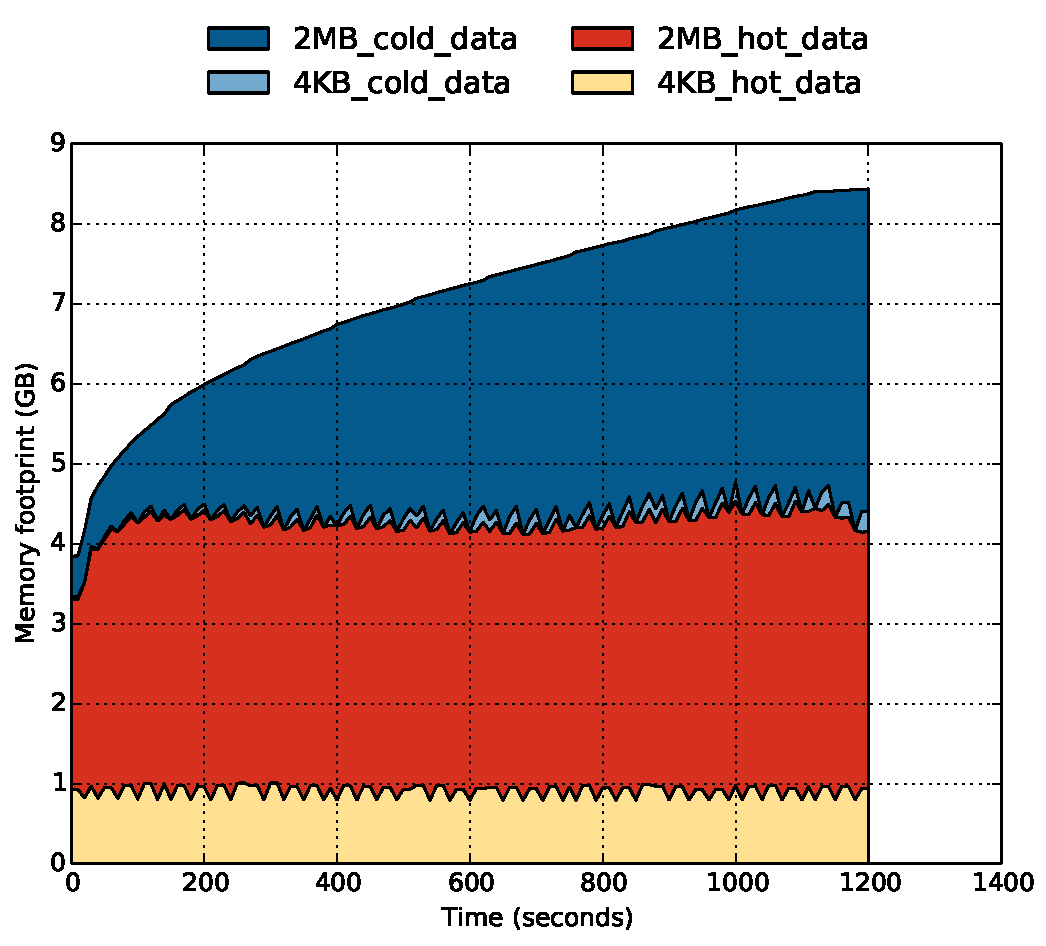
\includegraphics[width=0.8\columnwidth]{asplos2017/figures/tpcc-clipped-new-policy-capacity_over_time.pdf}
\caption{Amount of cold data in MySQL-TPCC identified at run time with 1.3\%
throughput degradation.}
\label{fig:tpcc-capacity}
\end{figure}

\begin{figure}[t]
\centering
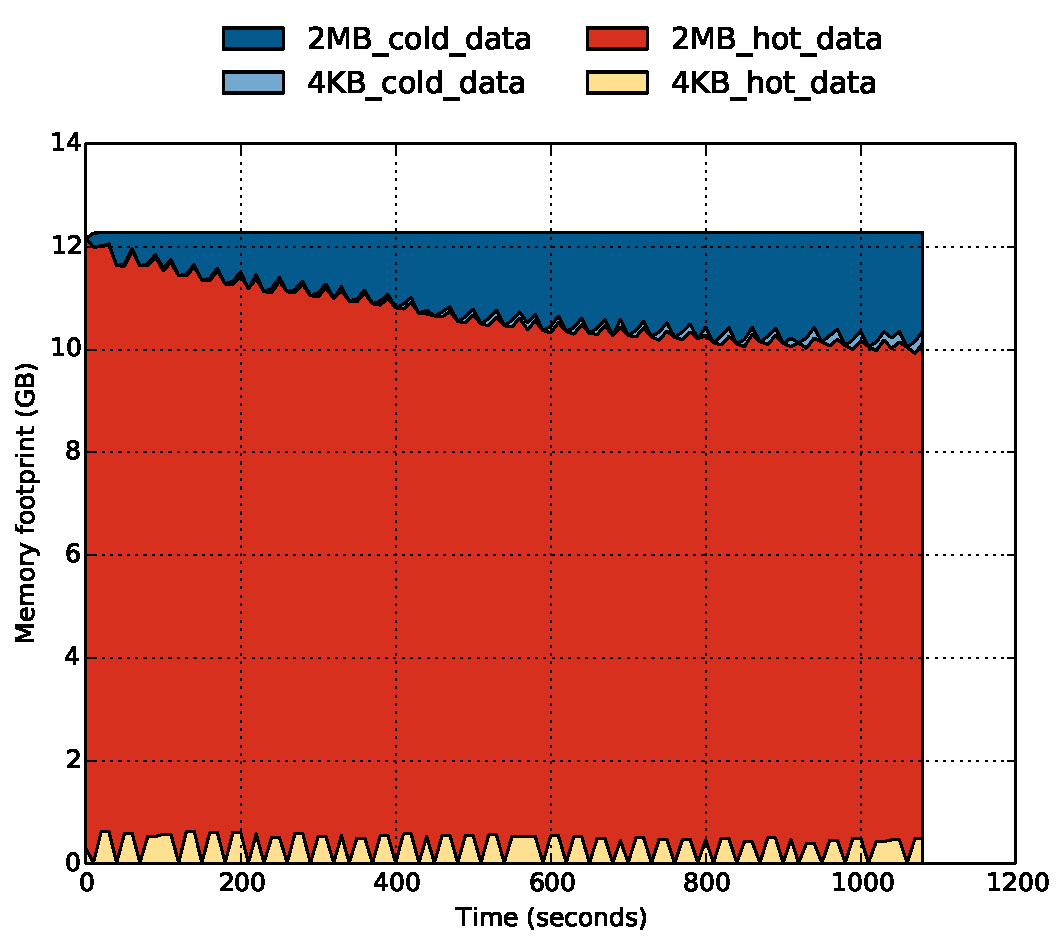
\includegraphics[width=0.8\columnwidth]{asplos2017/figures/aero-new-policy-24perSlow-capacity_over_time.pdf}
\caption{Amount of cold data in Aerospike identified at run time with 1\%
throughput degradation for a read-heavy workload (95:5 read/write ratio).}
\label{fig:aerospike-capacity}
\end{figure}

\begin{figure}[t]
\centering
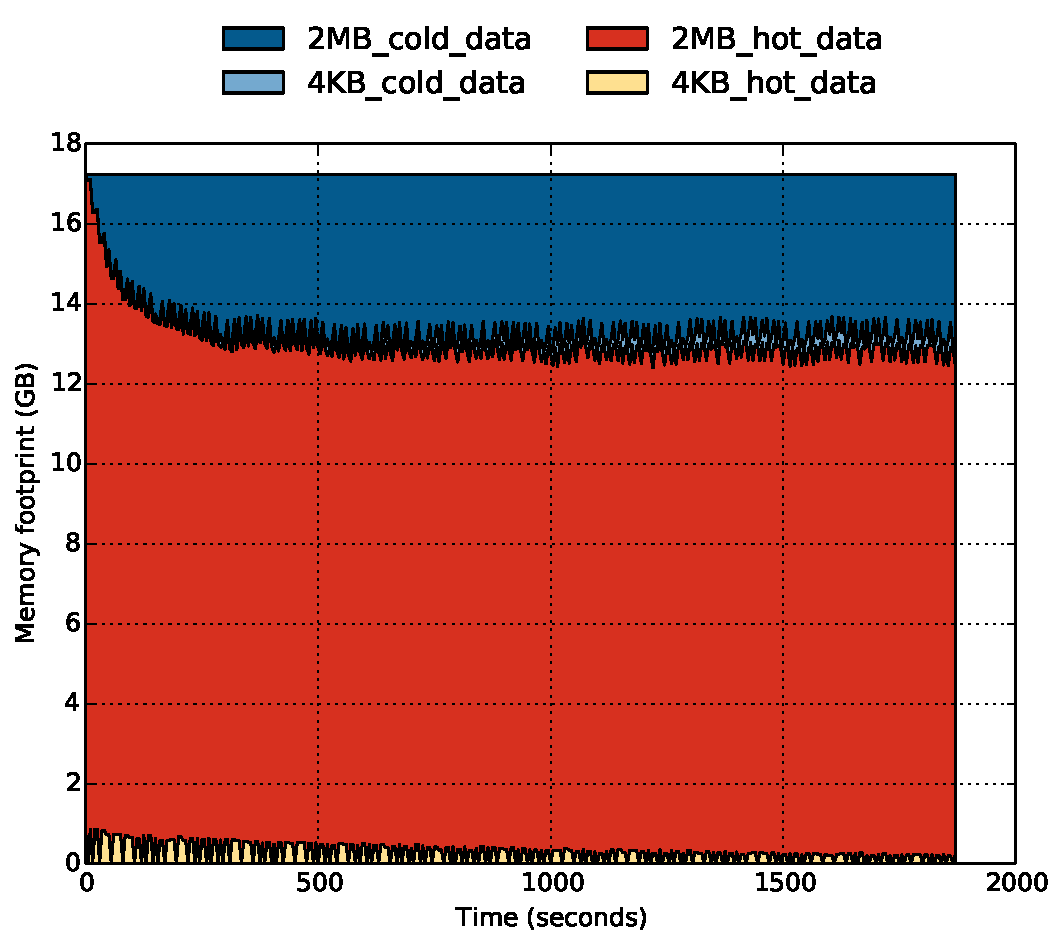
\includegraphics[width=0.8\columnwidth]{asplos2017/figures/redis-skewed-kstaled5-sample5-capacity_over_time.pdf}
\caption{Amount of cold data in Redis identified at run time with 2\%
throughput degradation.}
\label{fig:redis-skewed-hotspot-capacity}
\end{figure}

%\begin{figure}[t]
%\centering
%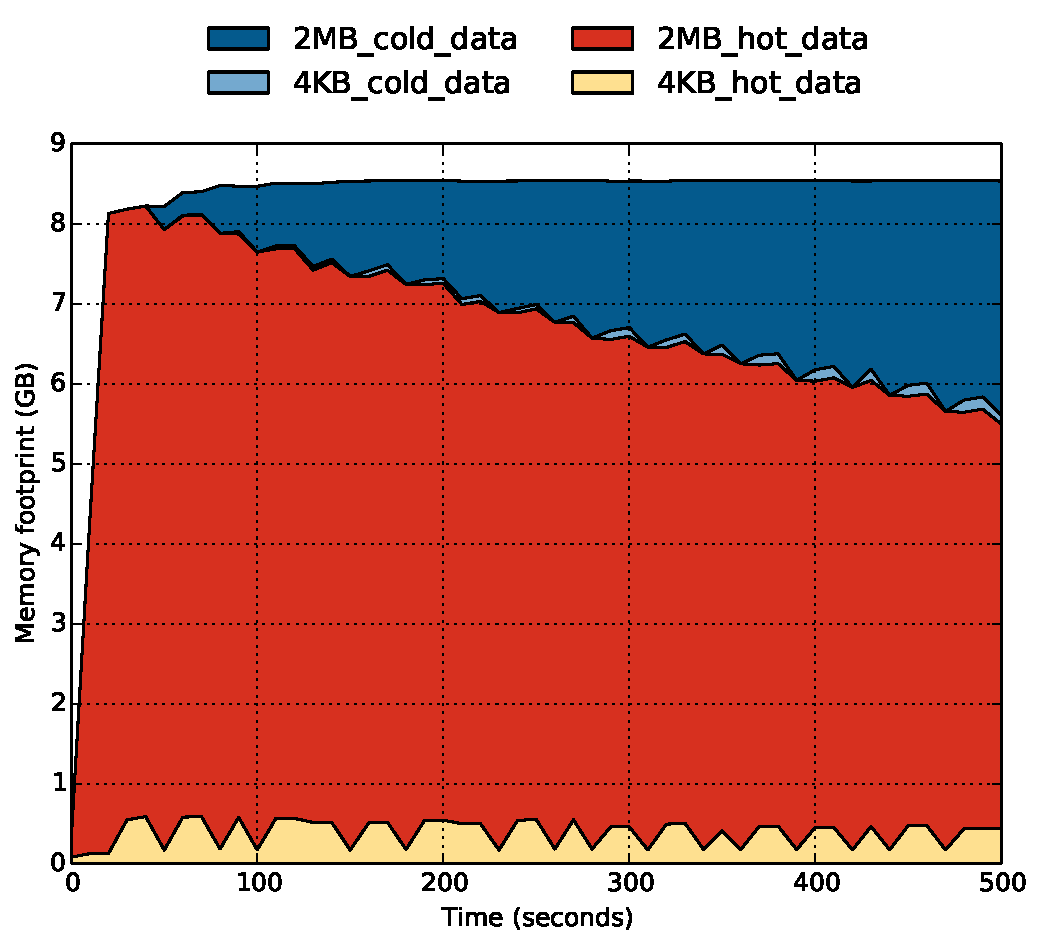
\includegraphics[width=1.0\columnwidth]{figures/ga-new-policy-36cpus-5iter-capacity_over_time.pdf}
%\caption{Amount of cold data in graph analytics benchmark identified at run time with 4\%
%runtime overhead.}
%\label{fig:graph-analytics-capacity}
%\end{figure}
%
\begin{figure}[t]
\centering
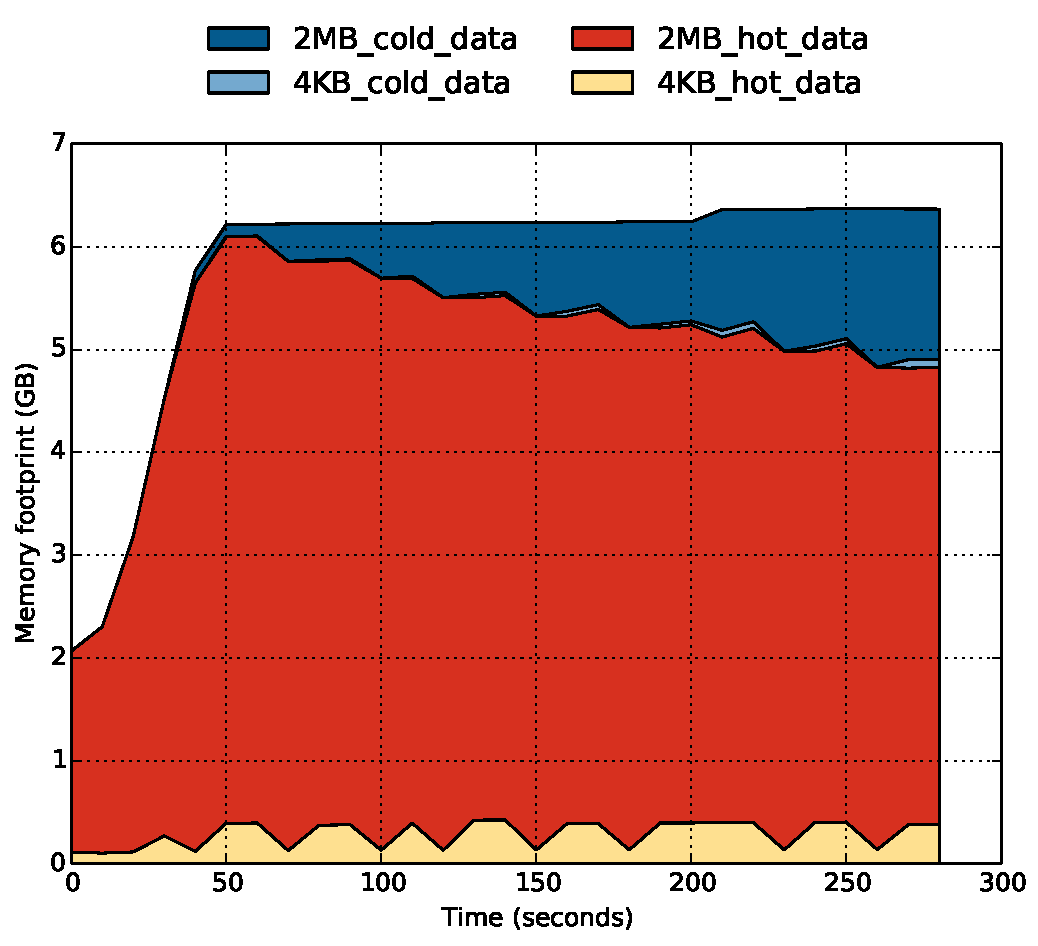
\includegraphics[width=0.8\columnwidth]{asplos2017/figures/ina-6g-new-policy-capacity_over_time.pdf}
\caption{Amount of cold data in in-memory analytics benchmark identified at run
time with 3\% runtime overhead.}
\label{fig:in-memory-analytics-capacity}
\end{figure}

\begin{figure}[t]
\centering
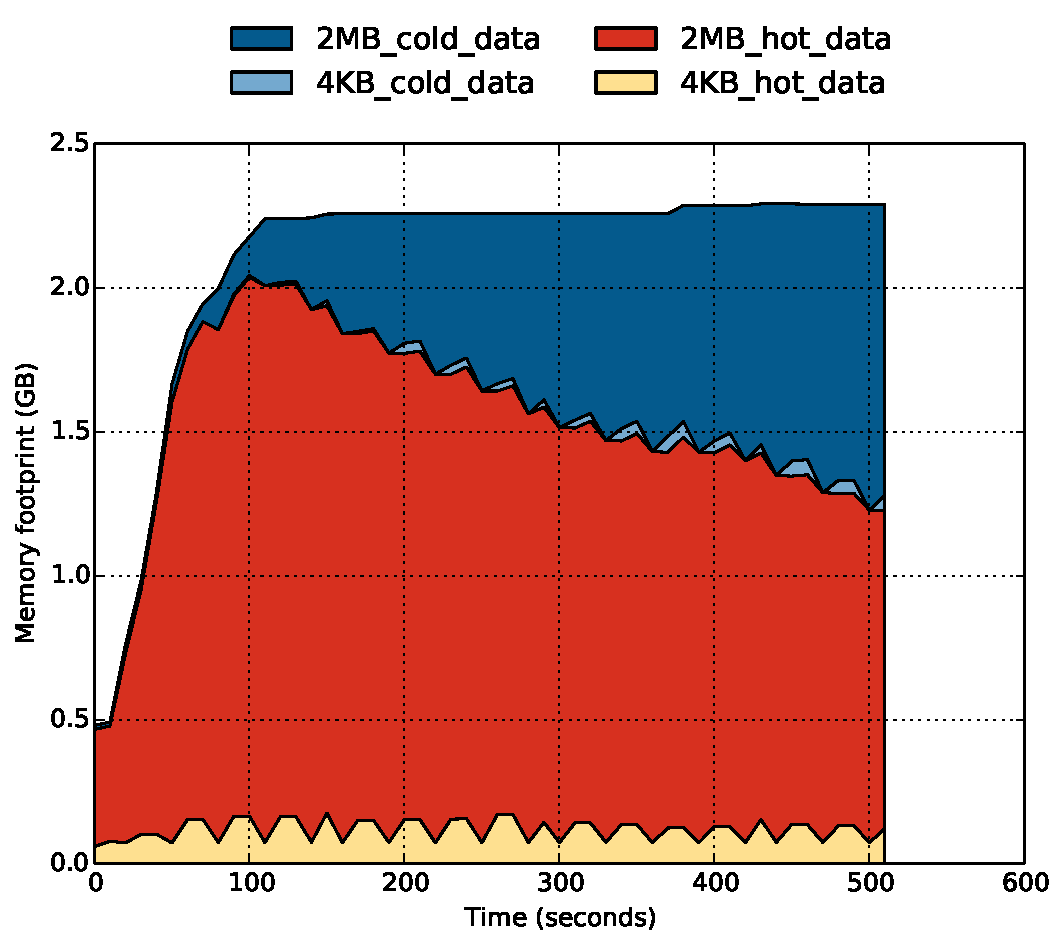
\includegraphics[width=0.8\columnwidth]{asplos2017/figures/wb-hugetmpfs-capacity_over_time.pdf}
\caption{Amount of cold data in web-search benchmark identified at run
time with 1\% throughput and no 99th percentile latency degradation.}
\label{fig:web-search-capacity}
\end{figure}

%\begin{figure}[t]
%\centering
%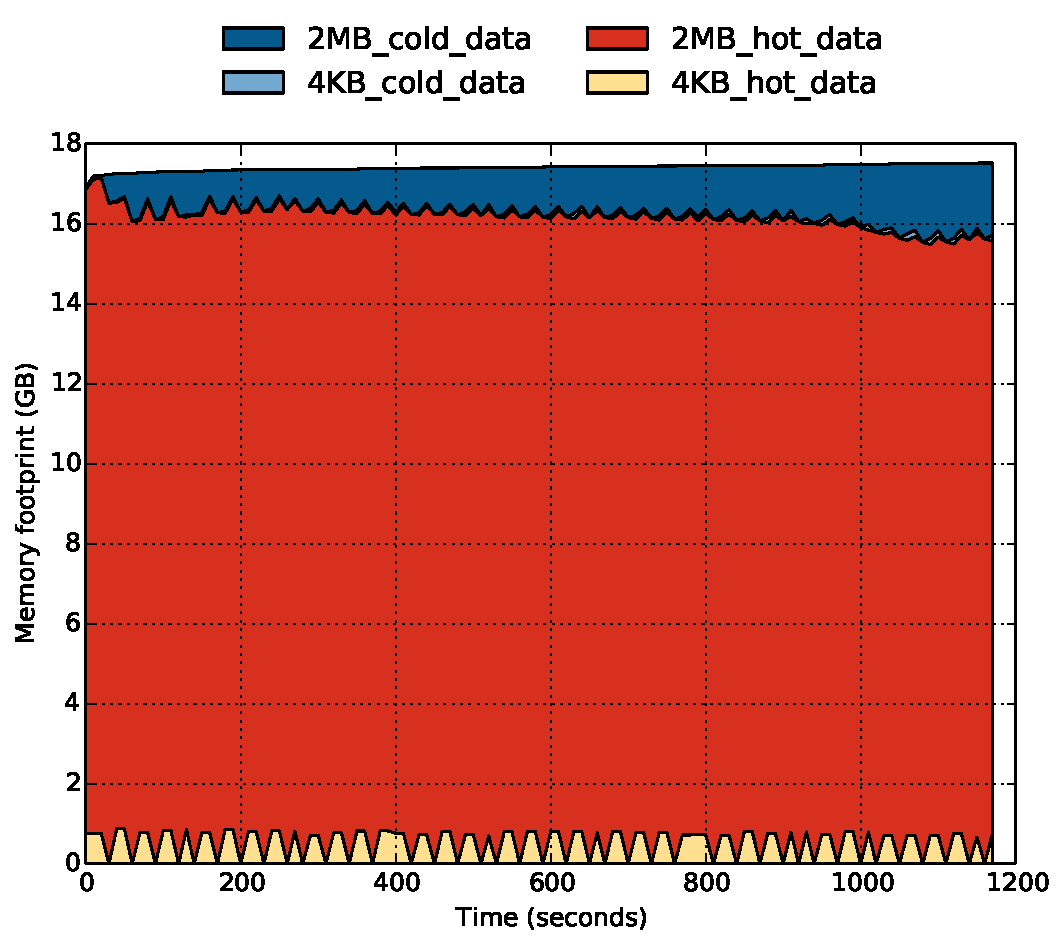
\includegraphics[width=1.0\columnwidth]{figures/redis-new-policy-normal-capacity_over_time.pdf}
%\caption{\fixme{Amount of cold data in Redis identified at run time with 3\%
%throughput degradation.}}
%\label{fig:redis-normal-hotspot-capacity}
%\end{figure}

\begin{figure}[t]
\centering
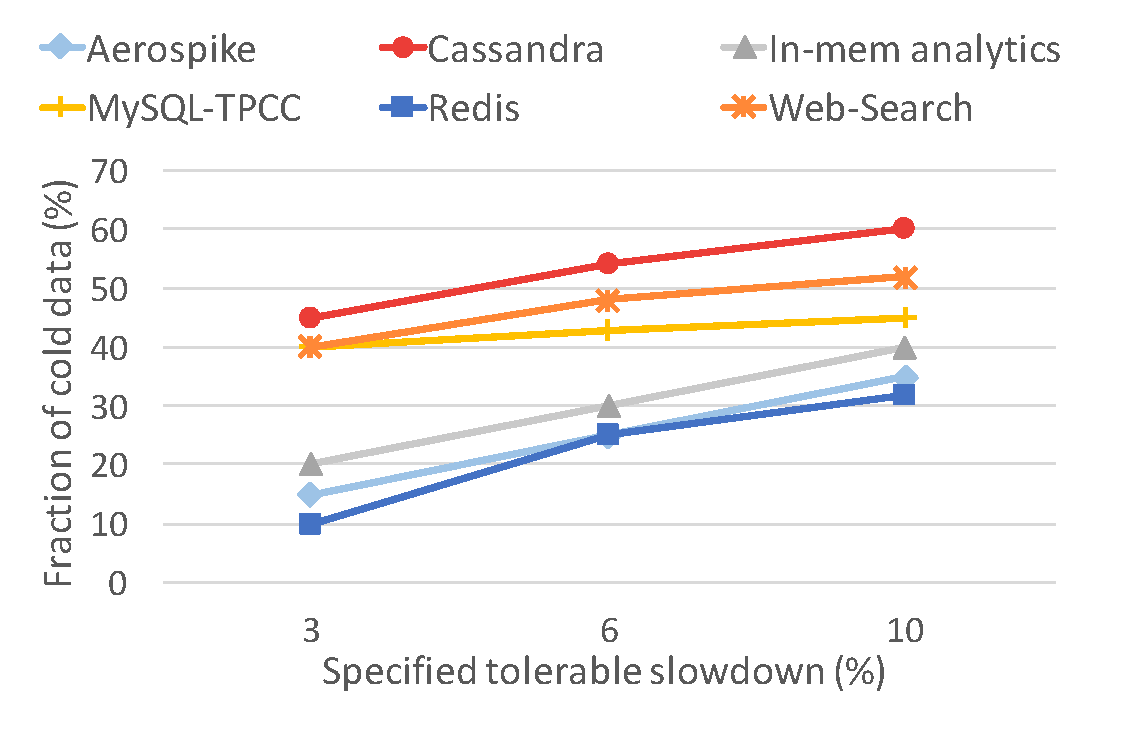
\includegraphics[width=0.8\columnwidth]{asplos2017/figures/slowdown-capacity-sweep.pdf}
\caption{Amount of cold data in identified at run
time varying with the specified tolerable slowdown. All the benchmarks meet
their performance targets (not shown in the figure) while placing cold data in
the slow memory.}
\label{fig:slowdown-capacity}
\end{figure}

%\subsection{Cassandra}
%\label{sec:cassandra}
\textbf{Cassandra}:
We report the breakdown of hot and cold 2MB and 4KB pages over time for 
Cassandra in Figure~\ref{fig:cassandra-capacity} for the write-heavy workload. 
Thermostat identifies between 40-50\% of Cassandra's footprint
(including both 4KB and 2MB pages) as cold. Note that the cold 4KB pages are
solely due to splitting of cold huge pages during profiling ($\approx$ 5\% of
cold pages are 4KB, since our profiling strategy is agnostic of a page being hot
or cold).
Note that the resulting throughput degradation of 2\% falls slightly under our 
target of 3\%. We observe $\approx$ 1\% higher average, 95th, and 99th percentile read/write
latency for Cassandra with Thermostat.
Based on this performance vs. footprint trade-off, we estimate Thermostat 
enables a net cost savings of $\approx$ 30\% for Cassandra (see
Section~\ref{dram-cost} for a detailed analysis). For the read-heavy workload
Thermostat identifies 40\% of data as cold with 2.5\% throughput degradation (we
omit figure due to space constraints).

The memory consumption of Cassandra grows due to in-memory Memtables filling up.
The Memtable is flushed to disk in the form of an SSTable, which then leads to a
sharp decrease in memory consumption. However, we do not observe such a
compaction event in our configuration, due to the large amount of memory
provisioned for Cassandra in our test scenario.

%A distinctive feature of Cassandra's memory footprint is the periodic sawtooth pattern
%visible in the Figure.
%This pattern continues indefinitely if we allow Cassandra to continue to run.
%Cassandra's footprint grows for a period of several hundred seconds as additional entries are 
%appended to its in-memory SSTable cache.  When SSTables grow to a pre-determined
%size, Cassandra invokes a compaction step that consolidates several SSTables into a 
%single file on disk and discards the stale files, leading to a sudden and sharp drop in its
%total footprint in the page cache. Note that the data in these SSTables is extremely cold.
%Hence, Cassandra benefits greatly from shifting a bulk of the page cache to huge pages
%in slow memory.

%\subsection{MySQL-TPCC}
%\label{sec:tpcc}
\textbf{MySQL-TPCC}:
In Figure~\ref{fig:tpcc-capacity} we show a similar footprint graph for MySQL-TPCC. 
The largest table
in the TPCC schema, the LINEITEM table, is infrequently read.  As a result, much
of TPCCs footprint (about 40-50\%) is cold and can be placed in slow memory while
limiting performance degradation to 1.3\%.

%\subsection{Aerospike}
\textbf{Aerospike}:
In Figure~\ref{fig:aerospike-capacity} we show a similar footprint graph for
Aerospike for the read-heavy workload. We see a small fraction of the footprint (about 15\%) identified
as cold while maintaining the tolerable slowdown. The average, 95th and 99th
read/write latencies are all within 3\% of the baseline. For the write-heavy
workload, Thermostat identifies about 15\% of data as cold while satisfying
tolerable slowdown (we omit figure due to space constraints).

%\subsection{Redis}
%\label{sec:redis}
\textbf{Redis}:
Unlike the other applications, Redis has a more uniform access pattern.
The key data structure in Redis is a large hash table, hence, memory accesses
are spread relatively uniformly over its address space; the relative hotness
of pages reflects the corresponding hotness of the key distribution.
We study a load where 0.01\% of keys account for 90\% of accesses.
In Figure~\ref{fig:redis-skewed-hotspot-capacity} we show that, under this load, 10\% of the data is detected as cold at a 3\% throughput degradation. 
The average read/write latency is 3.5\% higher than the baseline.
%There is small fraction of data idenitfied as cold for 3\% tolerable slowdown.
%The input key distribution is skewed, however, due to hashing hot keys are
%uniformly distributed across applicaiton pages. Hence, most pages are detected
%as hot, resulting in very low amount of cold data detection (about 10\%) for
%tolerable 3\% slowdown.

%However, in Figure~\ref{fig:redis-skewed-hotspot-capacity} we show that with a
%highly skewed access pattern as discussed in Section~\ref{sec:benchmarks},
%Thermostat can identify about 25\% as cold while being under tolerable 3\%
%slowdown.Thus, Thermostat successfully identifies cold pages if present in the
%application.

%\subsection{In-memory analytics}
\textbf{In-memory analytics}:
We also evaluate in-memory analytics benchmark from
Cloudsuite~\cite{cloudsuite}.  In Figure~\ref{fig:in-memory-analytics-capacity}
we show Thermostat detects about 15-20\% data as cold. As application footprint
grows, Thermostat scans more pages and thus the cold page fraction also grows with time.
We run this benchmark to completion, however, the benchmark runtime is much shorter
than the previous data serving applications. (Cloudsuite is 
designed for tractable runtimes under expensive instrumentation and/or simulation). 
Nevertheless,  Thermostat successfully identifies cold data while meeting the
slowdown target.  We expect the cold memory footprint of this application to 
reach steady state if a larger input were available.

%\subsection{Web search}
\textbf{Web search}:
In Figure~\ref{fig:web-search-capacity} we show the footprint graph for the web search workload. We see about 40\% of the footprint identified as cold. 
We observe $<$ 1\% degradation in throughput and no observable degradation in 99th
percentile latency of 200ms.

%\subsection{Sensitivity to hot-cold classification}
%To form a more complete picture of the trade-off between the fraction of memory
%classified as cold and performance degradation, we sweep a range of Thermostat
%classification thresholds and report the resulting trade-offs in Figure~\ref{fig:throughput-capacity}.
%The horizontal access reports the fraction of memory classified as cold while the
%vertical axis reports the corresponding throughput degradation for each of the three
%applications.
%
%TPCC is relatively insensitive to main memory access latency.  It incurs less than 
%5\% throughput degradation even when mapping 90\% of data to slow memory.
%%\fixme{Doesn't this result sort of imply your classification sucks?  Shouldn't you be classifying more stuff as cold?  This result seems awfully fishy.}
%In contrast, Redis is extremely sensitive to main memory access latency, slowing
%by more than 10\% if more than 40\% of its memory footprint is classified as cold.
%Cassandra is relatively tolerant of slower memory access except for about 20\%
%of its footprint, which is extremely hot and incurs drastic slowdown if shifted
%to slow memory.
%
%Figure~\ref{fig:cdf-sample2} also shows that Redis has two categories of
%pages (corresponding to two steep slopes in the CDF): one colder category with
%$\approx$ 100-200 hot 4KB pages, and another hotter category with $\approx$
%300-400 hot 4KB pages. Na\"{\i}vely, one would assume that the entirety of the
%``cold''-er data can be placed in slow memory. However, an accurate evaluation with our
%evaluation methodology shows that only about 40\% of that memory can actually be
%mapped to slow memory without suffering significant throughput degradations --
%highlighting the utility of an application-transparent and
%hardware-investment-free approach.
%

%\subsection{Sensitivity to tolerable slowdown}
%
%\subsection{Sensitivity to slow memory latency}
%\begin{figure}[t]
%\centering
%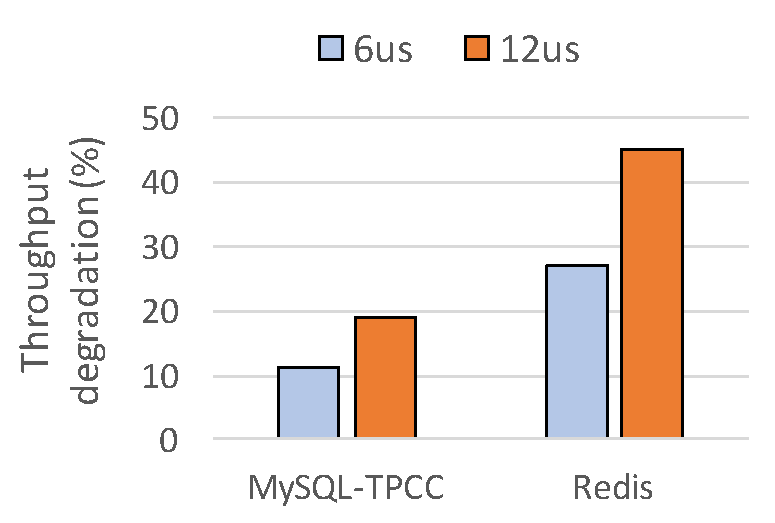
\includegraphics[width=1.0\columnwidth]{figures/latency-sweep.pdf}
%\caption{Slow memory latency sweep for 6 $\mu$s and 12 $\mu$s. Cassandra's throughput
%drops to 0 multiple times in between the run because of such high latencies.
%(Lower is better).}
%\label{fig:latency-sweep}
%\end{figure}
%
%As the access latency of future memory technologies remains uncertain, we perform
%a sensitivity study where we substantially increase the slow-memory access latency to
%6 and 12 microseconds.  We select these values to represent prior work on 
%disaggregated memory~\cite{Lim2012} where slow-memory accesses must 
%traverse a high-latency interconnect. Figure~\ref{fig:latency-sweep} shows the resulting 
%throughput degradation for Redis and TPCC. Cassandra fails to complete under these
%settings, due to application timeouts, so we omit its results. We can see that whereas TPCC can
%withstand a memory latency of 6 $\mu$s with $<$ 10\% throughput
%degradation, none of the applications can withstand 12 $\mu$s slow memory
%latency without significant throughput degradation. This observation points to
%the unsuitability of cache-line-grained accesses for such high memory latencies.


\subsection{Sensitivity to tolerable slowdown target}
Next we show the sensitivity of Thermostat to the single input parameter
specified by a system administrator, the tolerable slowdown. In our baseline evaluation, we set this parameter to 3\%. However, due to changes in the
price point of the memory technology or changes in data-center cost structure
it may be  possible to tolerate higher slowdown. To study the adaptability of
Thermostat in such scenarios we also evaluate 6\% and 10\% slowdown targets. We show the variation in amount of cold data identified by
Thermostat at run time with tolerable slowdown in Figure~\ref{fig:slowdown-capacity}.

We observe that with increase in tolerable slowdown Thermostat can place a higher
fraction of memory footprint in slow memory. We also observe
that the performance targets of all applications are met (we omit data due to space
constraints). However, in several cases, the achieved slowdown is less than the
specified slowdown.
%For Redis, Thermostat is able to identify higher
%fraction of cold data for higher tolerable slowdown as well as observed slowdown
%tracks the specified tolerable slowdown.

For MySQL-TPCC, Thermostat is not able to identify additional cold data even with
an increase in tolerable slowdown (cold data fraction saturates at $approx$ 45\%).
This saturation happens because all remaining pages for TPCC are highly accessed, and
placing any of them in slow memory results in an unacceptable application
slowdown.
%due to a sharp increase in memory access rate of pages in the application, which
%if migrated to slow memory will result in slowdown beyond tolerable, violating
%performance guarantees.
For Aerospike, Thermostat is able to scale the cold data
with varying tolerable slowdown. However, the actual slowdown doesn't reach the
target slowdown due to (a) Aerospike's performance being insensitive to cold page
accesses, and (b) the average OS fault handler latency for emulation being lower
than the assumed latency of 1us used in Thermostat.
%We attribute this observation to the fact that slow memory latency
%emulated in our platform depends on the page fault handler latency whose latency
%is not exactly 1us (lower in case of Aerospike), forcing Thermostat to
%pessimestically place smaller fraction of application data in slow memory. Note
%that on a platform with physical slow memory this problem will not be exhibited.

In summary, Thermostat places a higher fraction of data in slow memory if
the user can tolerate more slowdown. This feature
allows system administrators to better utilize expensive DRAM capacity by moving
as much cold data to slow memory as possible via Thermostat.

\subsection{Migration overhead and slow memory access rate}
\begin{table}
\begin{center}
\begin{tabular}{|c|c|c|}
%\begin{tabular}{|p{0.25\columnwidth}|c|c|}
\hline
(MB/s)&Migration& False-classification\\
\hline
Aerospike & 13.3& 9.2\\
\hline
Cassandra & 9.6 & 3.8\\
\hline
%Graph-Analytics & 7.5& 0.9\\
%\hline
In-mem-Analytics & 16& 0.4\\
\hline
MySQL-TPCC & 6 & 1.8\\
\hline
Redis & 11.3& 10\\
\hline
Web-search & 1.6 & 0.3\\
\hline
\end{tabular}
\caption{Data migration rate and false classification rate of slow memory. These rates are
well-below expected bandwidth of near-future memory technologies.}
\label{tab:nvm-access-rate}
\end{center}
\vspace{-0.15in}
\end{table}

To verify that Thermostat doesn't cause un-realizable bandwidth pressure on the
slow memory, we measured the memory bandwidth required by migrations and false
classifications between slow and fast memory.  In
Table~\ref{tab:nvm-access-rate} we observe that the required migration bandwidth
is $<$ 30 MB/s on average across all benchmarks.  The highest total traffic to
cold memory we observe is 60 MB/s, which is well within the projected capability
of near-future cheap memory technologies~\cite{ref:Dulloor:datatiering}. Thus,
we infer that Thermostat doesn't produce unrealistic pressure on the memory
system.

\subsection{DRAM Cost Analysis}
\label{dram-cost}
Since DRAM pricing is volatile, and slow memory prices remain unclear, it is difficult
to perform a rigorous cost-savings analysis for Thermostat.  We use a simple
model to estimate the cost-savings possible with Thermostat and study a range of 
possible ratios of DRAM to slow-memory cost.
Table~\ref{tab:cost-analysis} shows the fraction of DRAM spending
saved due to Thermostat when slow memory is $\frac{1}{3}$, $\frac{1}{4}$ and
$\frac{1}{5}$ of DRAM cost. We can see that, depending on workload and memory
technology, anywhere from $\approx$ 10\% (for Aerospike) to 32\% (for Cassandra)
of DRAM cost can be saved.

\begin{table}
\begin{center}
\begin{tabular}{|p{0.35\columnwidth}|c|c|c|}
\hline
Slow memory cost relative to DRAM&$0.33\times$& $0.25\times$ & $0.2\times$\\
\hline
Aerospike & 10\% & 11\% & 12\% \\
\hline
Cassandra & 27\% & 30\% & 32\% \\
\hline
In-mem-Analytics & 11\% & 12\% & 13\% \\
\hline
MySQL-TPCC & 27\% & 30\% & 32\% \\
\hline
Redis & 17\% & 19\% & 20\% \\
\hline
Web-search & 27\% & 30\% & 32\% \\
\hline
\end{tabular}
\caption{Memory spending savings relative to an all-DRAM system when using slow
memory with different cost points relative to DRAM.}
\label{tab:cost-analysis}
\end{center}
\vspace{-0.15in}
\end{table}

